\section{Question 4}
Inertia:
$$
I_x = 8, \quad I_y=10, \quad I_z = 14
$$

$$
\sigma_x = \dfrac{I_y-I_z}{I_x} = -0.5, \quad \sigma_z = \dfrac{I_y-I_x}{I_z} = 0.1429
$$

$$
\omega_0 = \sqrt{\dfrac{\mu}{R_0^3}} = 0.0011
$$

The characteristic equation of system is:
\begin{equation}
    s^4   + \omega_0^2(3s^2\sigma_x + \sigma_x\sigma_y + 1)  +4\,{\omega_0 }^4 \,\sigma_x \,\sigma_z = s^4 - 6.998\times10^{-07} s^2 - 3.499\times10^{-7}
\end{equation}

poles of the system ploted if figure \ref{poles}.

\begin{figure}[H]\label{poles}
    \caption{poles of system}
    \centering
    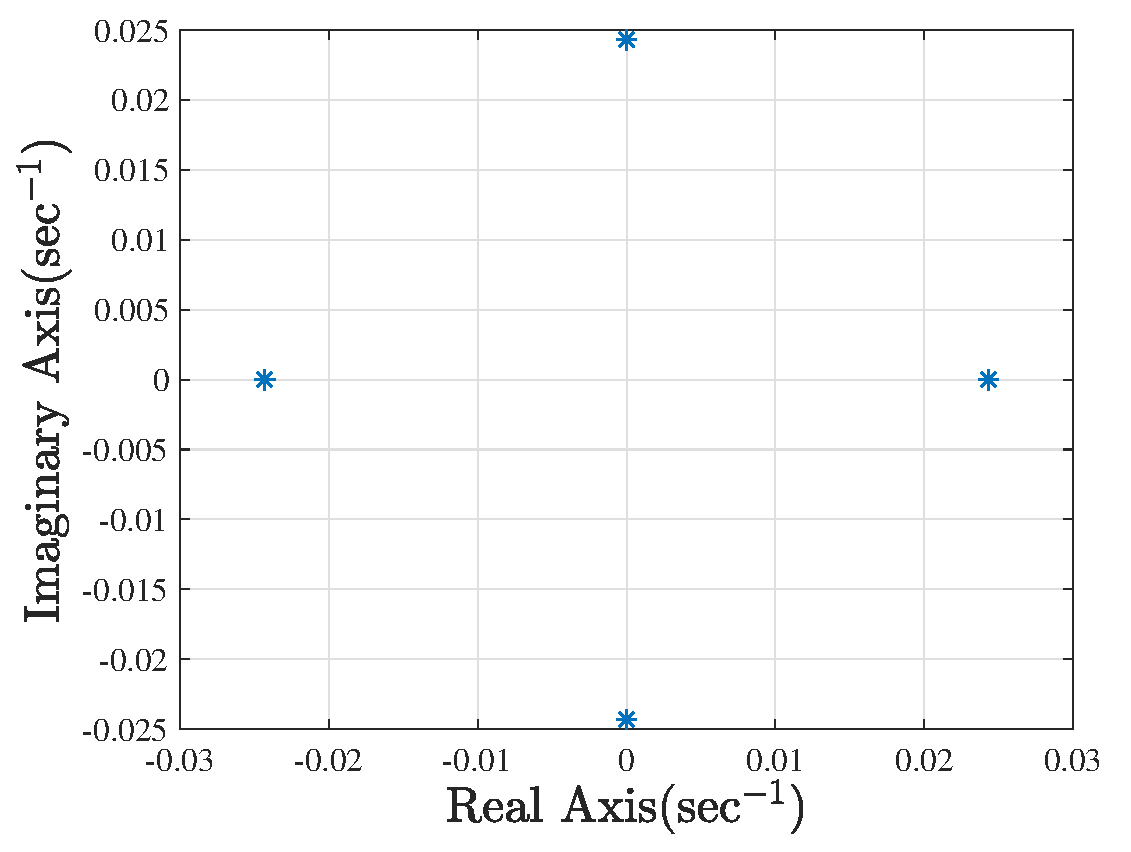
\includegraphics[width=12cm]{../Figure/Q4/pole_zero_map}
\end{figure}

Beacuse system has poles in right side of real axis, system is unstable and we have seen it in question 2.

